\documentclass[preprint,12pt]{elsarticle}
\usepackage{geometry}
%\geometry{letterpaper}                   % ... or a4paper or a5paper or ...
\usepackage{graphicx}
\usepackage{xspace}
\usepackage{amssymb} 
\usepackage{epstopdf}
\usepackage{graphicx,color}

 
\usepackage{datatool}
\usepackage{tikz}
\usepackage{pgfplots}
\usepackage{pgfplotstable}
\usetikzlibrary{patterns}
\usepackage{lscape}
\usepackage{subfig}

%% Use the option review to obtain double line spacing
%% \documentclass[preprint,review,12pt]{elsarticle}
   
%% Use the options 1p,twocolumn; 3p; 3p,twocolumn; 5p; or 5p,twocolumn
%% for a journal layout: 
%% \documentclass[final,1p,times]{elsarticle}
%% \documentclass[final,1p,times,twocolumn]{elsarticle}
%% \documentclass[final,3p,times]{elsarticle}
%% \documentclass[final,3p,times,twocolumn]{elsarticle}
%% \documentclass[final,5p,times]{elsarticle}
%% \documentclass[final,5p,times,twocolumn]{elsarticle}

%% if you use PostScript figures in your article
%% use the graphics package for simple commands
%% \usepackage{graphics}
%% or use the graphicx package for more complicated commands
%% \usepackage{graphicx}
%% or use the epsfig package if you prefer to use the old commands
%% \usepackage{epsfig}

%% The amssymb package provides various useful mathematical symbols
\usepackage{amssymb}
%% The amsthm package provides extended theorem environments
%% \usepackage{amsthm}

%% The lineno packages adds line numbers. Start line numbering with
%% \begin{linenumbers}, end it with \end{linenumbers}. Or switch it on
%% for the whole article with \linenumbers after \end{frontmatter}.
%% \usepackage{lineno}

%% natbib.sty is loaded by default. However, natbib options can be
%% provided with \biboptions{...} command. Following options are
%% valid:

%%   round  -  round parentheses are used (default)
%%   square -  square brackets are used   [option]
%%   curly  -  curly braces are used      {option}
%%   angle  -  angle brackets are used    <option>
%%   semicolon  -  multiple citations separated by semi-colon
%%   colon  - same as semicolon, an earlier confusion
%%   comma  -  separated by comma
%%   numbers-  selects numerical citations
%%   super  -  numerical citations as superscripts
%%   sort   -  sorts multiple citations according to order in ref. list
%%   sort&compress   -  like sort, but also compresses numerical citations
%%   compress - compresses without sorting
%%
%% \biboptions{comma,round}

% \biboptions{}


\journal{Journal of Systems and Software}

%%% OUR MACROS %%%
\newcommand{\COMMENT}[1]{ }

%\usepackage[usenames,dvipsnames]{xcolor}
\usepackage{xcolor}


\usepackage{amsmath}
\usepackage[thmmarks,amsmath]{ntheorem}

\newcommand{\openbox}{\leavevmode
  \hbox to.77778em{%
  \hfil\vrule
  \vbox to.675em{\hrule width.6em\vfil\hrule}%
  \vrule\hfil}}

\theoremstyle{plain}
\theoremheaderfont{\normalfont\bfseries}
\theorembodyfont{\normalfont}
\theoremseparator{}
\theoremindent0cm
\theoremnumbering{arabic}
\newtheorem{algo}{Algorithm}

\theoremstyle{plain}
%\theoremheaderfont{\normalfont\itshape}
\theoremheaderfont{\normalfont\bfseries}
\theorembodyfont{\normalfont}
\theoremseparator{}
\theoremindent0cm
\theoremnumbering{arabic}
\theoremsymbol{\ensuremath{\openbox}} 
\newtheorem{example}{Example}


\theoremstyle{plain}
\theoremheaderfont{\normalfont\bfseries}
\theorembodyfont{\normalfont}
\theoremseparator{.}
\theoremindent0cm
\theoremnumbering{arabic}
\theoremsymbol{\ensuremath{\Box}} 
\newtheorem{defi}{Definition}

\theoremstyle{plain} 
\theoremsymbol{\ensuremath{\Box}} 
\theoremseparator{.} 
\newtheorem{prop}{Property}

\usepackage{listings}


\lstset{numbers=right, numbersep=5pt, numberstyle=\tiny, stepnumber=1,escapechar=\!,columns=fullflexible,
        morekeywords={procedure,let,for,do,if,then,else,add,choose,end,while,
        true,false,rise,exception,extend,resume,to,return,function}}

\begin{document}

\begin{frontmatter}

%% Title, authors and addresses

%% use the tnoteref command within \title for footnotes;
%% use the tnotetext command for the associated footnote;
%% use the fnref command within \author or \address for footnotes;
%% use the fntext command for the associated footnote;
%% use the corref command within \author for corresponding author footnotes;
%% use the cortext command for the associated footnote;
%% use the ead command for the email address,
%% and the form \ead[url] for the home page:
%%
%% \title{Title\tnoteref{label1}}
%% \tnotetext[label1]{}
%% \author{Name\corref{cor1}\fnref{label2}}
%% \ead{email address}
%% \ead[url]{home page}
%% \fntext[label2]{}
%% \cortext[cor1]{}
%% \address{Address\fnref{label3}}
%% \fntext[label3]{}

\title{SLA-based Data Integration on Multi-Cloud: A Systematic Mapping Analysis}

%% use optional labels to link authors explicitly to addresses:
%% \author[label1,label2]{<author name>}
%% \address[label1]{<address>}
%% \address[label2]{<address>}



\author[inst1]{Daniel Aguiar}
\author[inst2]{Nadia Bennani}
\author[inst1]{Chirine Ghedira}
\author[inst4]{Pl\'acido A. Souza Neto}
\author[inst5]{Genoveva Vargas-Solar}

 
%\address[inst4]{Universidad de las Am\'ericas-Puebla, LAFMIA -- Cholula, Mexico}
\address[inst1]{Universit\'e Jean Moulin, Lyon 3 MAGELLAN, IAE -- France}
\address[inst2]{CNRS INSA-Lyon, LIRIS, UMR5205 -- France}
\address[inst4]{Instituto Federal do Rio Grande do Norte, Natal -- Brazil}
\address[inst5]{CNRS, LIG-LAFMIA, Saint Martin d'H\`eres -- France} 
  
\begin{abstract}

\ldots
\end{abstract}

\begin{keyword}
%% keywords here, in the form: keyword \sep keyword
\ldots \sep \ldots \sep Systematic Mapping.

%% MSC codes here, in the form: \MSC code \sep code
%% or \MSC[2008] code \sep code (2000 is the default)

\end{keyword}

\end{frontmatter}

%%
%% Start line numbering here if you want
%%
% \linenumbers

%% main text
%*********************************************************************************************************

%-[BEGIN]-----------------------------------------------------------------------
\section{Introduction}
\label{sec:intro}
\section{Introduction}
\label{sec:intro}

%\idaniel{Doing Nadia's request, I've checked for works regarding our three keywords and also their variations and I didn't find anything. But I found one using Grid "SLA-Guided Data Integration on Database Grids".}

The emergence of new architectures like the cloud opens new opportunities to data processing. 
The possibility of having unlimited access to cloud resources and the ``pay as U go'' model make it possible to change the hypothesis for processing big  data collections.  Instead of designing processes and algorithms taking into consideration  limitations on resources availability, the cloud sets the focus on the economic cost implied of using resources and producing results by parallelizing their use while delivering data under subscription oriented cost models.
 
Integrating and processing heterogeneous Big Data, calls for efficient methods for correlating, associating, filtering them taking into consideration their ``structural'' characteristics (due to variety) but also their quality (veracity), e.g., trust, freshness, provenance, partial or total consistency. 
Existing data integration techniques have to be revisited considering weakly curated and modeled data sets. This can be done according to quality of service requirements expressed by their consumers and Service Level Agreement (SLA) contracts exported by the cloud providers that host  Big Data and deliver resources for executing the associated management processes.

However, it is not an easy task to completely fulfill   SLA contracts particularly because they have to use several cloud providers to integrate the data they require under the conditions they expect.
Naturally, a collaboration between cloud providers becomes necessary~\cite{036} but this should be done in a user-friendly way, with high degree of transparency. As result, new challenges emerge.

SLA have been widely discussed in the cloud computing context. ...

Data Integration...


Our work addresses big data collections integration  in a multi-cloud hybrid context guided by user preferences statements and SLA contracts exported by different cloud providers. The objective is to propose an SLA guided continuous data provision and integration system exported as a DaaS by a cloud provider adapted to the vision of the economic model of the cloud such as accepting partial results delivered on demand or under predefined subscription models that can affect the quality of the results; accepting specific data duplication that can respect privacy but ensure data availability; accepting to launch a task that contributes to an integration on a first cloud whose SLA verifies a QoS require



In this paper, we propose an analysis about the problem of integrating data in multi-cloud environments taking into consideration Service Level Agreement. 
The methodology defined in~\cite{SM:Petersen:2008} presents some guidelines to
performing a systematic mapping review in software engineering research
context. The systematic mapping is a defined method to build
a classification of a field of interest. The results analysis focuses on
frequencies of publications for categories (facets).  

The process workflow describes five interdependent tasks: \textit{(i)}
\textbf{definition of research question} to define the \textit{research scope}; \textit{(ii)} textbf{conduct search} in order to retrieve \textit{all candidate papers}. Those papers are selected applying a query which
express the research interest to scientific databases; \textit{(iii)}
\textbf{screening of papers} to select the \textit{relevant papers} to answer the research
question based on a inclusion and exclusion criteria; \textit{(iv)}
\textbf{keywording using abstracts} to identify terms that helps on developing the
\textit{classification scheme} (mapping categories to classify the papers); and
\textit{(v)} \textbf{fata extraction and mapping process} to sort the relevant
papers into the mapping categories and produce the systematic mapping.


This analysis was done using the Systematic Mapping Methodology~\cite{SM:Petersen:2008}. We propose three facets to determine the main issues to be addressed when SLA, Data Integration and Multi-cloud environments are put together in one research problem.

%The methodology consists in retrieving publications from scientific databases and classifying them in
%categories (called facets). As result we have charts which are used to answer specific research questions
%created in accordance with scientific interests. 


Our final objective is to identify trends and open issues regarding our research topic.

The remaining of this paper is organized as follows. 
The related work is in the section~\ref{sec:rw}. 
section~\ref{sec:sm} describes our steps regarding the methodology.
A quantitative analysis based on the facets is discussed in the section~\ref{sec:qanalysis} and conclusion and final
remarks comes in the section~\ref{sec:conc}. 
%-[END]-----------------------------------------------------------------------
%-[BEGIN]-----------------------------------------------------------------------
\section{Related Works}

\subsection{Data integration on multi-cloud environment}

\subsection{Service level agreement}
%-[END]-----------------------------------------------------------------------


%-[BEGIN]-----------------------------------------------------------------------
\section{Systematic Mapping process}

The aim of our bibliographic study using the systematic mapping methodology \cite{SM:Petersen:2008} is to (i) categorize and quantify the key contributions and the evolution of the research done on \textit{SLA-guided
data integration in a multi-cloud environment} and  (ii) discover open issues and limitations of existing works.    
Our study is guided by  three research questions:


\textit{\textbf{RQ1:} Which are the SLA measures that have been mostly
applied  in the cloud?} This question  identifies  the type of
properties used for characterizing and evaluating the services provided  by
different clouds.   
 
\textit{\textbf{RQ2:}  How have published papers on data
 integration evolved towards cloud topics?} This question is devoted to identify the way  data integration problems addressed in the literature started  to include issues introduced by the cloud.

\textit{\textbf{RQ3:} In which way and in which  context has data integration  been linked to Quality of Service (QoS) measures in the literature?} The objective of this question is to understand which QoS measures have been used for evaluating data integration and to determine the conditions in which  specific measures are particularly used.

%--------------------------------------------------------------------------------------------------------------------------------------------
\subsection{Searching and screening  papers} \label{subsec:search}
%--------------------------------------------------------------------------------------------------------------------------------------------

According to our research questions and our expertise in data integration we chose a set of keywords to define a complex query to be used for retrieving papers from four target publication databases: IEEE~\footnote{http://ieeexplore.ieee.org/},
ACM~\footnote{http://dl.acm.org/}, Science Direct~\footnote{http://www.sciencedirect.com/} and
CiteSeerX~\footnote{http://citeseerx.ist.psu.edu/}. We used the following conjunctive and disjunctive general query which was completed with associated terms from a thesaurus and rewritten according to the expression rules of advanced queries in each database: 




\begin{center}
\textit{("Service level agreement"  AND ("Data integration" OR "Database
integration") AND ("Cloud" OR "Multi-cloud "))} \\
\end{center}
\medskip  

We retrieved  a total of 1832 publications. As a result of the filtering process
proposed by the systematic mapping methodology~\cite{SM:Petersen:2008} we excluded 1718 publications.
The number of papers included for building the final collection were 114
publications~\footnote{List of references available in:
https://github.com/danielboni/DEXA-2015-Can-Data-Integration-Quality-be-Enhanced-on-Multi-cloud-using-SLA.git}.

%--------------------------------------------------------------------------------------------------------------------------------------------
\subsection{Defining classification facets}
%--------------------------------------------------------------------------------------------------------------------------------------------

We analyzed the titles and abstracts of the  papers derived in the previous
phase using information retrieval techniques  to identify  frequent
 terms. We used these terms for proposing a classification scheme
consisting of three facets that group dimensions. The following lines define the facets and dimensions of the
classification scheme we propose. 

%.  -   .  .  -   ..  -   ..  -   ..  -   ..  -   ..  -   ..  -   ..  -   ..  -   ..  -   ..  -   ..  -   ..  -   ..  -   ..  -   ..  -   ..  -   ..  -   ..  -   ..  -   ..  -   ..  -   ..  -   .  
\textbf{\textit{Data Integration Environment:}}  
%.  -   .  .  -   ..  -   ..  -   ..  -   ..  -   ..  -   ..  -   ..  -   ..  -   ..  -   ..  -   ..  -   ..  -   ..  -   ..  -   ..  -   ..  -   ..  -   ..  -   ..  -   ..  -   ..  -   ..  -   .  
This facet groups the dimensions that characterize the architectures used for delivering data integration services ({\em data warehouse} and  {\em federated database}) and  architectures used for deploying these services ({\em cloud} and {\em multi-cloud}).

%.  -   .  .  -   ..  -   ..  -   ..  -   ..  -   ..  -   ..  -   ..  -   ..  -   ..  -   ..  -   ..  -   ..  -   ..  -   ..  -   ..  -   ..  -   ..  -   ..  -   ..  -   ..  -   ..  -   ..  -   .  
\textbf{\textit{Data Integration Description:}}
%.  -   .  .  -   ..  -   ..  -   ..  -   ..  -   ..  -   ..  -   ..  -   ..  -   ..  -   ..  -   ..  -   ..  -   ..  -   ..  -   ..  -   ..  -   ..  -   ..  -   ..  -   ..  -   ..  -   ..  -   .  
 This facet groups the dimensions describing the approaches used for describing the databases content in order to  integrate them. Data integration can be done by using {\em meta-data, schema}, and {\em knowledge}.

%.  -   .  .  -   ..  -   ..  -   ..  -   ..  -   ..  -   ..  -   ..  -   ..  -   ..  -   ..  -   ..  -   ..  -   ..  -   ..  -   ..  -   ..  -   ..  -   ..  -   ..  -   ..  -   ..  -   ..  -   .  
\textbf{\textit{Data Quality:}} 
%.  -   .  .  -   ..  -   ..  -   ..  -   ..  -   ..  -   ..  -   ..  -   ..  -   ..  -   ..  -   ..  -   ..  -   ..  -   ..  -   ..  -   ..  -   ..  -   ..  -   ..  -   ..  -   ..  -   ..  -   .  
This facet groups the dimensions  representing data quality measures. Measures can be related directly to data for instance {\em confidentiality, privacy, security, protection and provenance} and to the conditions in which data is integrated and delivered  (i.e., dimension {\em SLA}).           

The original vision of our classification scheme is that of adding the notion of {\em quality} to data integration represented by the facets {\em data quality}
and  {\em SLA}.
With these facets our classification scheme shows the aspects that must be considered when addressing data integration in the cloud  taking into account (i) the quality of data, (ii) the systems that integrate data and (iii) the quality warranties that a data consumer can expect expressed in SLAs.

%------------------------------------------------------------------------------- %
\section{Quantitative Analysis}\label{sec:qanalysis}
%--------------------------------------------------------------------------------% 

This section discusses the quantitative analysis  presented in bubble charts that combine different facets. 
In order to observe the evolution of the publication trends we defined a time screen between the years 1998 and 2014 (see Figure \ref{fig:pubperyear}). SLA has emerged when Cloud issues started to be addressed around 2009. The number of publications has increased as cloud infrastructures have become more popular and accessible. It seems  that data integration is an open issue when it is combined with SLA and cloud trends. Less recent papers seem to be devoted to the way data is described under schemata or knowledge representation strategies. This could be due to the fact that these strategies are consolidated today and  to the emergence of NoSQL approaches with their schema-less philosophy \cite{sadalage2012nosql}. 

\begin{figure}[ht!]
\centering
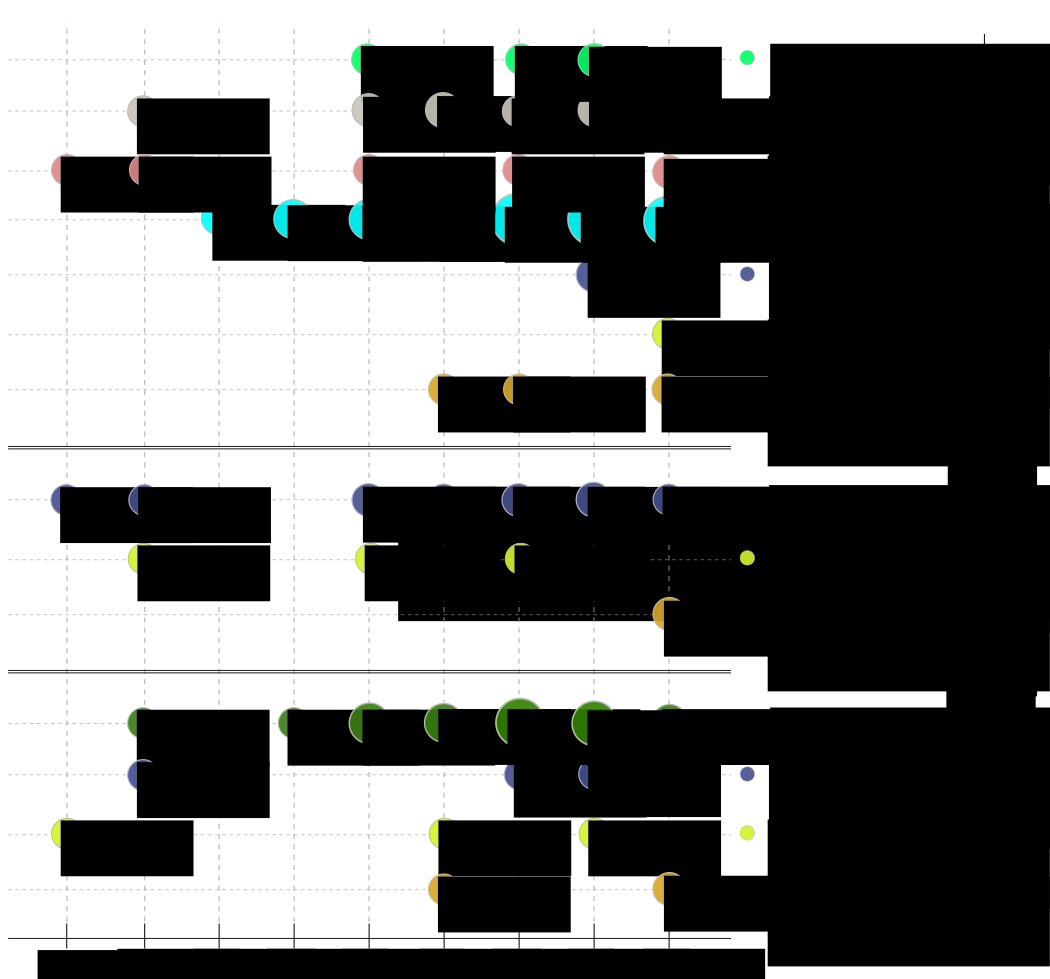
\includegraphics[scale=0.33]{figs/bubble-charts/PublicationsPerYear.pdf} 
\caption{Publications Per Year}\label{fig:pubperyear}
\end{figure}

We combined facets for answering the research questions proposed for guiding our
study. The following lines discuss the answers.
 
%  . .  .  . .  .  . .  .  . .  .  . .  .  . .  .  . .  .  . .  .  . .  .  . .  .  . .  .  . .  .  . .  .  . .  .  . .  .  . .  .  . .  .  . .  .  . .  .  . .  .  . .  .  . .  .
\textbf{\textit{RQ1: Which are the SLA measures that have been mostly applied 
in the cloud?}}
%  . .  .  . .  .  . .  .  . .  .  . .  .  . .  .  . .  .  . .  .  . .  .  . .  .  . .  .  . .  .  . .  .  . .  .  . .  .  . .  .  . .  .  . .  .  . .  .  . .  .  . .  .  . .  .


The facets SLA expression, data integration description and contribution give elements for determining which SLA measures have been applied to the cloud (Figure~\ref{fig:facet1}). 
The resulting bubble chart shows that most contributions propose SLA models and that  \textit{privacy}
and \textit{security} (11 papers - 9.65\%) are the most popular measures considered by SLA models for the cloud. These measures concern the network, information, data protection and confidentiality in the cloud. Most contributions propose SLA models (53 papers - 46.49\%)  but some languages (8 papers - 7.02\%) have also emerged. {\em Data provenance} is also a measure that emerges but only in papers dealing with multi-cloud environments. Data integration is merely addressed by using schemata (12 papers - 10.53\%)  and meta-data (4 papers - 3.51\%) particularly through models (34 papers - 29.82\%) and tools (25 papers - 21.93\%). Still, some works propose surveys (8 papers - 7.02\%).
 
\begin{figure}[ht!]
\centering
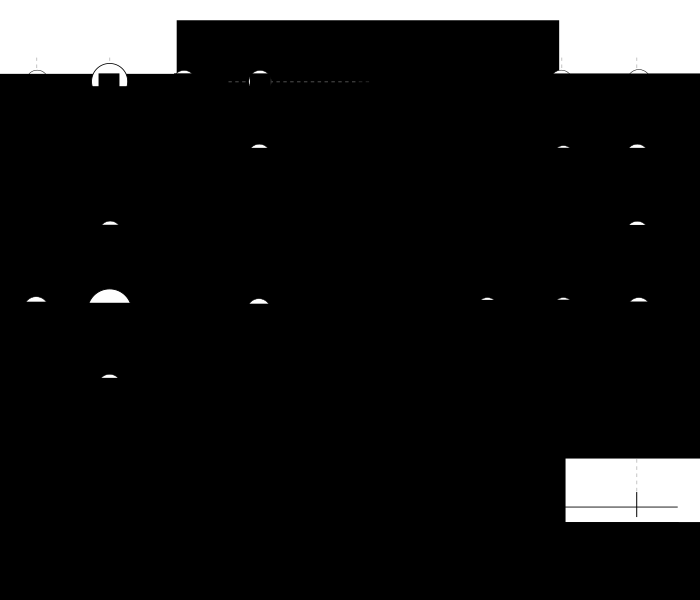
\includegraphics[width=0.75\textwidth]{figs/bubble-charts/Contribution-SLA-DIdescription.pdf}
  
\caption{Facets Contribution, SLA and Data Integration Description}\label{fig:facet1}
\end{figure} 

%  . .  .  . .  .  . .  .  . .  .  . .  .  . .  .  . .  .  . .  .  . .  .  . .  .  . .  .  . .  .  . .  .  . .  .  . .  .  . .  .  . .  .  . .  .  . .  .  . .  .  . .  .  . .  .
\textbf{\textit{RQ2: How have published papers on data integration evolved towards cloud topics?}}
%  . .  .  . .  .  . .  .  . .  .  . .  .  . .  .  . .  .  . .  .  . .  .  . .  .  . .  .  . .  .  . .  .  . .  .  . .  .  . .  .  . .  .  . .  .  . .  .  . .  .  . .  .  . .  .
\begin{figure}[h]
\centering
\includegraphics[width=0.86\textwidth]{figs/bubble-charts/DI-Environment-Contribution-Research.pdf}
\caption{Facets Data Integration Environment, Contribution and Research}\label{fig:facet2}
\end{figure}

Combining the facets data integration environment, contribution
and research it is possible to observe  the evolution of publications on data integration towards the cloud (Figure~\ref{fig:facet2}).  {\em Data warehouse} environments are the most common architecture. This can be explained by the increase of scientific  and industrial applications needing to build integrated  data sets for performing analysis and decision making tasks. The proposals are delivered as {\em models}  (14  papers - 12.27\%)  and {\em tools} (18
papers - 15.78\%)  used for facilitating data integration, mostly done in the {\em cloud}.  The most popular deployment environment of recent papers is the {\em cloud}. Given the importance and crucial need of data integration  most papers present concrete solutions as algorithms, methods and systems (31 papers - 27.19\%).
  
%  . .  .  . .  .  . .  .  . .  .  . .  .  . .  .  . .  .  . .  .  . .  .  . .  .  . .  .  . .  .  . .  .  . .  .  . .  .  . .  .  . .  .  . .  .  . .  .  . .  .  . .  .  . .  .
\textbf{\textit{RQ3:  In which way and in which context has data integration been linked to QoS measures in the literature?}}
%  . .  .  . .  .  . .  .  . .  .  . .  .  . .  .  . .  .  . .  .  . .  .  . .  .  . .  .  . .  .  . .  .  . .  .  . .  .  . .  .  . .  .  . .  .  . .  .  . .  .  . .  .  . .  .
\begin{figure}[!h]
\centering
\includegraphics[width=0.85\textwidth]{figs/bubble-charts/Data-Quality-DI.pdf}
\caption{Facets Data Quality, Data Integration Environment and Data Integration Description}\label{fig:facet4}
\end{figure}

We answered RQ3 by combining the facet {\em data quality} with the facets {\em data integration environment} and {\em data integration description}
(Figure~\ref{fig:facet4}).  Data integration and QoS measures are associated within environments like cloud  (9.68\%) and multi-cloud (4.39\%).

According to our quantitative analysis we observe that QoS has started to be
considered for integrating data. 
 The cloud is becoming a popular environment to
perform data integration in which security issues are most frequently addressed.
We identify a promising research area concerning the need of studying SLA which
is currently addressed  for the cloud as a whole \cite{PedrinaciCL14} but that
needs to be specialized for data integration aspects. Therefore, it is important
to identify the measures that characterize the quality of data and  the
quality measures associated to different phases of data integration. These phases include selecting
data services, retrieving data, integrating and correlating them and building a
query result that can be eventually stored and that must be delivered. The data integration phases are implemented by greedy algorithms and generate intermediate data that
can be stored for further use. Therefore they consume storage, computing,
processing and communication resources that have an associated economic cost. These resources 
 must ensure some QoS guarantees to data consumers. This problem seems to be
open in the domain, and we believe that it must be part of  a new vision of data
integration. We believe that it is possible to add and enhance the quality of
data integration by including SLAs.                   

%-[END]-----------------------------------------------------------------------
%-[BEGIN]-----------------------------------------------------------------------
\section{Quantitative Analysis}
\section{Quantitative Analysis}

\subsection{Combining the facets Contribution, SLA Usage and Data Integration Description}

\begin{figure}[h!]
\centering
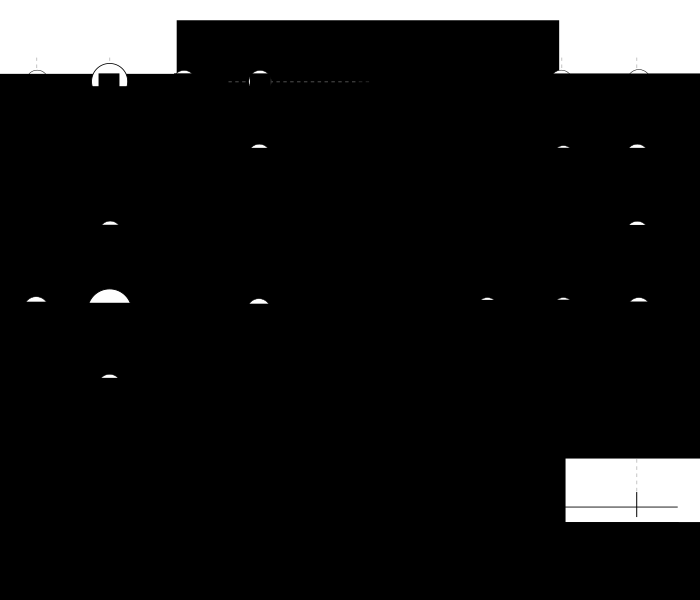
\includegraphics[scale=0.5]{figs/bubble-charts/Contribution-SLA-DIdescription.pdf} 
\caption{...}
\end{figure}

\subsection{Combining the facets Data Integration Environment, Contribution and Research}

\begin{figure}[h!]
\centering
\includegraphics[scale=0.5]{figs/bubble-charts/DI-Environment-Contribution-Research.pdf}
\caption{...}
\end{figure}

\subsection{Combining the facets SLA Usage and Contribution}

\begin{figure}[h!]
\centering
\includegraphics[scale=0.7]{figs/bubble-charts/SLA-Contribution.pdf}
\caption{...}
\end{figure}


\subsection{Combining the facets Data Quality, Data Integration Environment and Data Integration Description}

\begin{figure}[h!]
\centering
\includegraphics[scale=0.53]{figs/bubble-charts/Data-Quality-DI.pdf}
\caption{...}
\end{figure}

%-[END]-----------------------------------------------------------------------
%-[BEGIN]-----------------------------------------------------------------------
\section{Considering SLA and Data Integration on Multi-Cloud}
%-[END]-----------------------------------------------------------------------



%-[BEGIN]-----------------------------------------------------------------------
\section{Conclusion and final remarks}
 %-[END]-----------------------------------------------------------------------

%% References with bibTeX database:

\bibliographystyle{plain}
 \bibliography{bibliography,publications}


\end{document}

%%
%% End of file `elsarticle-template-1a-num.tex'.
